\documentclass[border=14pt]{standalone}
\usepackage{tikz}
\usetikzlibrary{arrows.meta, patterns}

\begin{document}
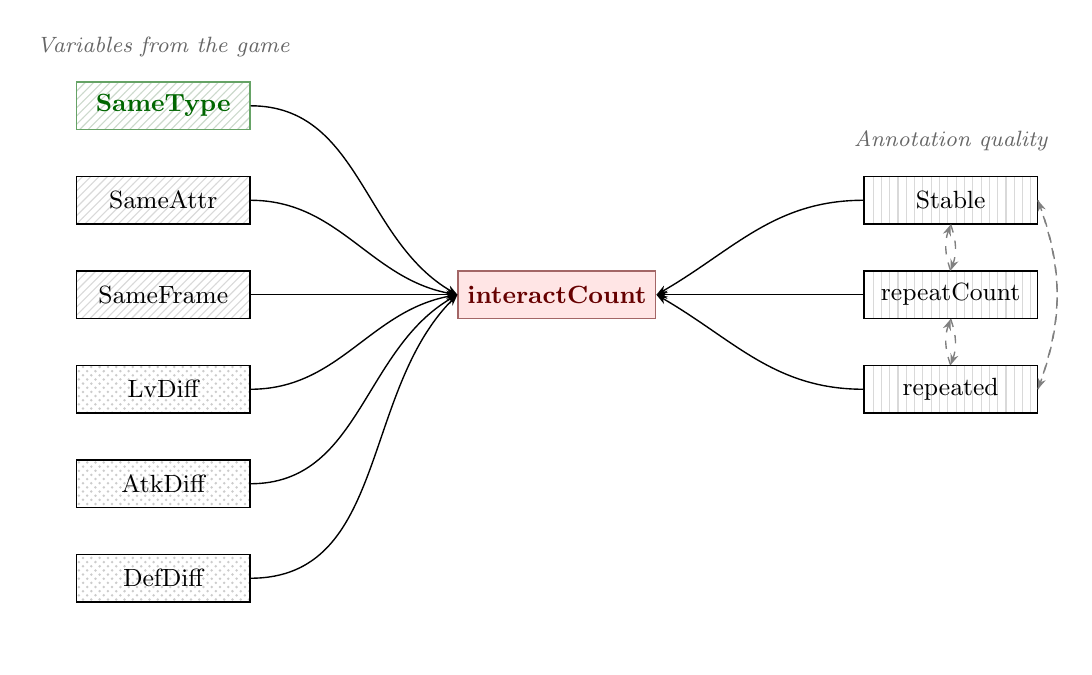
\begin{tikzpicture}[
    box/.style={
        rectangle, minimum width=2.2cm, minimum height=0.6cm,
        text centered, font=\small,
        draw=black, line width=0.5pt
    },
    box1/.style={box, fill=black!8,
        pattern=north east lines, pattern color=black!15},
    box1highlight/.style={box, fill=green!10!white,
    pattern=north east lines, pattern color=green!25!black!20,
    draw=green!40!black!60, 
    font=\small\bfseries, text=green!40!black},
    box2/.style={box, fill=black!5,
        pattern=crosshatch dots, pattern color=black!20},
    box3/.style={box, fill=black!8,
        pattern=vertical lines, pattern color=black!15},
    outcome/.style={box, fill=red!10!white, pattern color=red!25!black!20,
    draw=red!40!black!60, 
    font=\small\bfseries, text=red!40!black},
    darr/.style={
        -{Stealth[length=4pt, width=3pt]},
        line width=0.5pt, dashed, gray
    },
    arr/.style={
        -{Stealth[length=4pt, width=3pt]},
        line width=0.5pt, black
    }
]

\node[outcome] at (0,0)   (outcome) {interactCount};

\node[box1highlight] at (-5, 2.4)  (st)  {SameType};
\node[box1]          at (-5, 1.2)  (sa)  {SameAttr};
\node[box1]          at (-5, 0.0)  (sf)  {SameFrame};

\node[box2] at (-5,-1.2)  (lv)  {LvDiff};
\node[box2] at (-5,-2.4)  (atk) {AtkDiff};
\node[box2] at (-5,-3.6)  (def) {DefDiff};

\node[box3] at (5, 1.2)   (stb) {Stable};
\node[box3] at (5, 0.0)   (rpn) {repeatCount};
\node[box3] at (5,-1.2)   (isr) {repeated};

\draw[arr] (st.east)  to[out=0,  in=150] (outcome.west);
\draw[arr] (sa.east)  to[out=0,  in=170] (outcome.west);
\draw[arr] (sf.east)  --                  (outcome.west);
\draw[arr] (lv.east)  to[out=0,  in=190] (outcome.west);
\draw[arr] (atk.east) to[out=0,  in=210] (outcome.west);
\draw[arr] (def.east) to[out=0,  in=225] (outcome.west);

\draw[arr] (stb.west) to[out=180, in=30]  (outcome.east);
\draw[arr] (rpn.west) --                   (outcome.east);
\draw[arr] (isr.west) to[out=180, in=-30] (outcome.east);

\draw[darr, bend left=20]  (stb.south) to (rpn.north);
\draw[darr, bend left=20]  (rpn.north) to (stb.south);
\draw[darr, bend left=20]  (rpn.south) to (isr.north);
\draw[darr, bend left=20]  (isr.north) to (rpn.south);
\draw[darr, bend left=20] (stb.east) to (isr.east);
\draw[darr, bend right=20]  (isr.east) to (stb.east);

\node[font=\footnotesize\itshape, text=black!60] at (-5, 3.15) {Variables from the game};
\node[font=\footnotesize\itshape, text=black!60] at (-5,-4.35) {};
\node[font=\footnotesize\itshape, text=black!60] at (5,  1.95) {Annotation quality};


\end{tikzpicture}
\end{document}